\documentclass[tikz,border=8pt]{standalone}
\usepackage{amsmath,amssymb}
\usepackage{tikz}
\usetikzlibrary{patterns,shapes,positioning}

\begin{document}

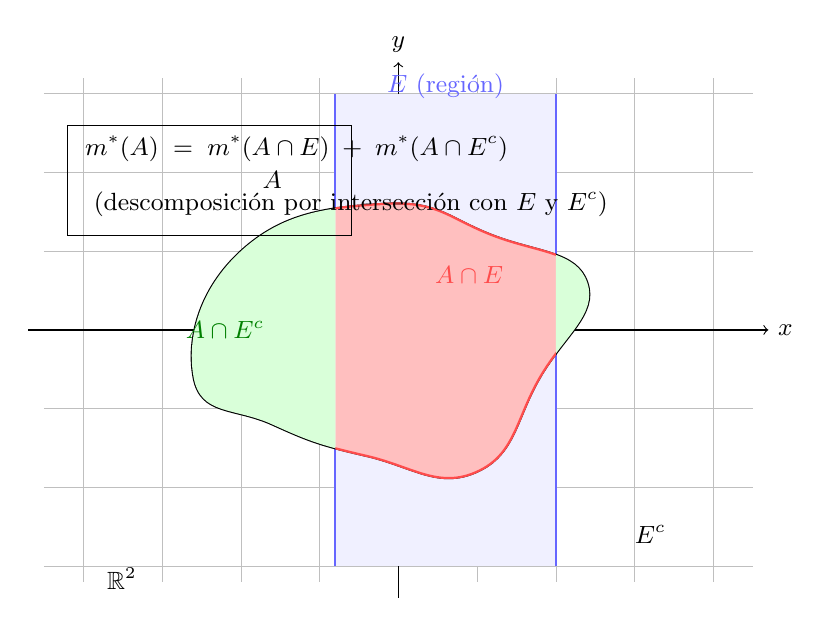
\begin{tikzpicture}[scale=1, every node/.style={font=\small}]
  % Axes
  \draw[gray!50, very thin] (-4.5,-3.2) grid (4.5,3.2);
  \draw[->] (-4.7,0) -- (4.7,0) node[right] {$x$};
  \draw[->] (0,-3.4) -- (0,3.4) node[above] {$y$};

  % Region E: a vertical strip (so E and E^c easy to visualise)
  \fill[blue!6] ( -0.8,-3) rectangle ( 2.0,3); % E shaded lightly
  \draw[blue!60, thick] (-0.8,-3) -- (-0.8,3) (2.0,-3) -- (2.0,3); % E boundaries
  \node[blue!60] at (0.6,3.1) {$E$ (región)};

  % Set A: an irregular blob (opaque outline)
  \begin{scope}
    \clip (-3.5,-2.5) rectangle (4.5,3.2); % limit drawing area
    \draw[fill=gray!5, draw=black, thick] 
      plot[smooth cycle, tension=0.8] coordinates {(-2.6,-0.6) (-2.0,1.0) (-0.2,1.6) (1.2,1.2) (2.4,0.6) (1.8,-0.6) (1.0,-1.8) (-0.4,-1.6) (-1.6,-1.2)} 
      node[pos=0.45] (Alabel) {}; % main A outline
  \end{scope}
  \node at (-1.6,1.9) {$A$};

  % Highlight A \cap E (portion of A inside the vertical strip)
  \begin{scope}
    \clip (-0.8,-3) rectangle (2.0,3); % restrict to E
    \fill[red!25] 
      plot[smooth cycle, tension=0.8] coordinates {(-2.6,-0.6) (-2.0,1.0) (-0.2,1.6) (1.2,1.2) (2.4,0.6) (1.8,-0.6) (1.0,-1.8) (-0.4,-1.6) (-1.6,-1.2)};
    % outline on top
    \draw[red!70, thick] 
      plot[smooth cycle, tension=0.8] coordinates {(-2.6,-0.6) (-2.0,1.0) (-0.2,1.6) (1.2,1.2) (2.4,0.6) (1.8,-0.6) (1.0,-1.8) (-0.4,-1.6) (-1.6,-1.2)};
  \end{scope}
  \node[red!70] at (0.9,0.7) {$A\cap E$};

  % Outline A cap E^c (portion of A outside the strip)
  \begin{scope}
    \clip (-4.5,-3) rectangle (-0.8,3); % left complement
    \fill[green!15] 
      plot[smooth cycle, tension=0.8] coordinates {(-2.6,-0.6) (-2.0,1.0) (-0.2,1.6) (1.2,1.2) (2.4,0.6) (1.8,-0.6) (1.0,-1.8) (-0.4,-1.6) (-1.6,-1.2)};
  \end{scope}
  \begin{scope}
    \clip (2.0,-3) rectangle (4.5,3); % right complement
    \fill[green!15] 
      plot[smooth cycle, tension=0.8] coordinates {(-2.6,-0.6) (-2.0,1.0) (-0.2,1.6) (1.2,1.2) (2.4,0.6) (1.8,-0.6) (1.0,-1.8) (-0.4,-1.6) (-1.6,-1.2)};
  \end{scope}
  \node[green!50!black] at (-2.2,0.0) {$A\cap E^c$};

  % Legend box with measure equality
  \draw[black] ( -4.2, 2.6) rectangle (-0.6, 1.2);
  \node[anchor=west] at (-4.1,2.3) {\(\displaystyle m^*(A)\;=\; m^*(A\cap E)\;+\; m^*(A\cap E^c)\)};
  \node[anchor=west] at (-4.1,1.6) {\(\) (descomposición por intersección con \(E\) y \(E^c\))};

  % small labels to show complement
  \node at (3.2,-2.6) {\(E^c\)};
  \node[below left] at (-3.2,-2.9) {\(\mathbb{R}^2\)};
\end{tikzpicture}

\end{document}
